\documentclass[11pt, a4paper, oneside]{report}
\usepackage{mathtools}
\usepackage{amsfonts}
\usepackage{minted}
\usepackage{booktabs}
\usepackage[UKenglish]{babel}
\usepackage[en-GB,showdow]{datetime2}
\usepackage{csquotes}
\usepackage{hyperref}
\usepackage{imakeidx} \makeindex
\usepackage[
sorting=none,
hyperref=true,
backend=biber,
style=numeric,
backref=true
]{biblatex}
\addbibresource{references.bib}
\usepackage{todonotes}
\usepackage{pdfpages}
\usepackage{glossaries} \makeglossaries
\usepackage{graphicx}
\usepackage{framed}
\usepackage{dsfont}
\usepackage{caption}
\usepackage{parskip}



\newglossaryentry{term}{ name={term}, description={``a
    word or expression that has a precise meaning in some uses or is
    peculiar to a science, art, profession, or
    subject'\autocite{dictionary:_term_defin_term} --- here text
    analysts have capitalised on the generalisation of ``term'to
    include subcomponents or aggregations of words} }




\begin{document}

% \frontmatter
\begin{titlepage}
  \centering
  \vspace*{2.5cm}
  {\Huge Text Analytics}\\
  \vspace{1.5cm}
  {\Large Jason Peter Cairns}\\
  \vspace{1.5cm}
  Supervised by Chris Wild\\
  \vspace{1.5cm}
  \begin{figure}[H]
    \centering
    
\includegraphics[scale=0.4]{img/logo.jpg}
  \end{figure}
  \vspace{1cm}
  Bachelor of Science (Honours)\\
  Department of Statistics\\
  The University of Auckland\\
  New Zealand
\end{titlepage}

\listoftodos

% \begin{abstract}

% \end{abstract}

\chapter*{Acknowledgements}
\label{cha:acknowledgements}

\tableofcontents
\addcontentsline{toc}{chapter}{Listings}
\renewcommand\listoflistingscaption{List of source codes}
\listoflistings
\addcontentsline{toc}{chapter}{Tables}
\listoftables
\addcontentsline{toc}{chapter}{Figures}
\listoffigures

% \mainmatter
\chapter{Introduction}
\label{cha:introduction}

\section{Intention}
\label{sec:intention}

Text Analytics serves to glean insight from a body of text. Within the
broad category of text analytics, we seek to answer questions about
what the text is communicating, what is felt about it, and how this
information is structured. In this dissertation, we demonstrate the
creation of a user-friendly program to perform text analytics
functions using modern R with the Shiny web application framework. In
a literate style, we illustrate top-down the structure of such a
program, as well as the data structures and computational processes
that have established their value for such a program.\todo{should this
  be an abstract?}
  
\section{Background: Text Analytics (incl. examples)}
\label{sec:backgr-text-analyt}
\subsection{common functions: sentiment, summarisation, scoring}
Text Analytics is comprised of a variety of processes and techniques
to extract information from text. The text almost always requires some
initial processing. Some of the following functions have proven
utility, and are expanded upon in \autoref{cha:text-analyt-backgr};

\begin{itemize}
\item Sentiment: In order to answer what emotions are conveyed in a
  text, sentiment analysis is commonly performed. The technique yields
  some measure of what is represented in an emotional sense by the
  text, with a range different methods and their associated outputs
  allowing for different forms of the analysis. Sentiment analysis
  won't pick up the subtle nuances that a human reader would, but
  generally gives reasonable output over the extent of a text.
\item Associated Words: The meaning of a text is dependent on the
  structure between and within words. Looking at how words are
  associated, through correlation, common sequences, visualisation of
  sections, etc.,\ allow for a clear high-level assessment of the
  associations between words. The higher level not only saves
  individual efforts, but will demonstrate any emergent properties
  inherent to a text, in a way that a direct reading won't necessarily
  reveal.
\item Summarisation: Automation of an executive summary, or a list of
  key words, typically falls under the purview of summarisation. The
  primary aim is to rank and select the most ``representative'' words
  or sentences from a text. A few major techniques dominate, being
  somewhat complex in nature. The results are generally surprisingly
  well representative of a text.
\item Feature Counts: The simplest quantitative measure is very often
  the most informative; from simple word counts, to selective counts
  of sentences within groups, counting features can reveal how much
  written weighting is given to various elements, aiding insight into
  both structure and sentiment simultaneously.
\end{itemize}

\subsection{Existing Systems}
There are several existing systems in the field of Text Analytics. The
field was initially nurtured as a sub-field of Computer Science, being
computationally-dependent in nature. More recently, there has been
increasing statistical interest. The existing systems reflect this;
most older text analytics programs were Artificial Intelligence
focussed, being experimental in nature, typically composed in lisp.
More recently, major statistical programs hae been incorporating text
analytic features, with a few smaller text analytics specific programs
appearing. SAS, SPSS, and R are all examples of major statistical
processing systems, with recent additions of text analytics
capabilities. An overview of R packages aiding in text analytics will
be given in \autoref{sec:liter-revi-exist}

\subsection{current issues}

\section{Background: inZight}
\label{sec:background:-inzight}
\subsection{What iNZight is - capabilities, popularity, etc.}
\subsection{how our program fits in - shiny, inzight lite etc.}

\section{Literature Review (existing packages in R)}
\label{sec:liter-revi-exist}

\subsection{Copy over from notes, flesh out a bit}
\subsection{Praise tidytext book, complain about the package}

\section{Scope of work}
\label{sec:scope-work}

\subsection{types of text that we can work with: novels, free response data etc.}
\subsection{discuss limitations placed: not going into linguistic territory etc.}

\chapter{Text Analytics Prolusion}
\label{cha:text-analyt-backgr}

\section{overview}
\label{sec:overview}
Most importantly, words must be extracted, serving as the basic unit
of analysis, from which more complex items may be derived.
\subsection{Explain broadness of term}
\subsection{compile glossary from terms here}
\subsection{Areas of text analytics in a data science framework}
\subsection{what we have done}
\subsection{what we haven't done}

\section{terms}
\label{sec:terms}
\gls{term}
\subsection{terms and their centrality}
\subsection{generalisation: n-grams, sentences etc.}

\section{Historical Background}
\label{sec:hist-backgr}

\subsection{computer science vs statistics - reflection in data science}

\section{Processing}
\label{sec:processing}

\subsection{why process}
\subsection{stopwords, lemmatisation etc.}
\subsection{modelling vs db joins - more info in notes}

\section{scores \& statistics}
\label{sec:statistics}

\subsection{why compute scores \& statistics}
\subsection{scoring - tf-idf, word count}
\subsection{Suggestions for further research - more on the statistics of words}
\subsection{recount the book of John text analysis}

\section{Sentiment}
\label{sec:sentiment}

\subsection{why sentiment}
\subsection{Process of sentiment}
\subsection{sentiment modelling vs db joins}
\subsection{our implementation and why}
\subsection{reviews}
\subsection{issues}

\section{Summarisation}
\label{sec:summarisation}

\subsection{why compute summarisations}
\subsection{lexrank, textrank - include notes on lexrank}
\subsection{other methods}
\subsection{reddit bot example}

\section{what we didn't do (yet)}
\label{sec:what-we-didnt}

\subsection{topic modelling}
\subsection{Term correlation}
\subsection{modelling based on linguistic features}

\section{Visualisation}
\label{sec:visualisation-1}

\subsection{talk about score vs structure}
\subsection{complain about tag clouds}
\subsection{talk about ggpage}
\subsection{discuss our experimentations with some alternative visualisations}
\chapter{Program Structure \& Development}
\label{cha:program-structure}

\subsection{why R}
\subsection{Why Shiny}
\subsection{why tidyverse}
\subsection{Git}
\subsection{possible future: datatables, futures, etc.}
\subsection{why functional}
\subsection{Why lossless data}

\section{Program Architecture}
\label{sec:program-architecture-1}

\subsection{Why structure it like it has been}
\subsection{make graph of architecture}
\subsection{Describe package and package creation}
\subsection{following three sections copy and paste from the notes - buffing up as necessary}
\subsection{include screenshots}

\section{Import}
\label{sec:import}

\section{Insight}
\label{sec:insight}

\section{Visualisation}
\label{sec:visualisation}

\section{User Interface}
\label{sec:user-interface}

\chapter{Conclusion}
\label{cha:conclusion}

\section{Summary}
\label{sec:summary}

\subsection{summarise successes}
\subsection{summarise failures}
\subsection{general thoughts on the topic}

\section{Recommendations}
\label{sec:recommendations}

\subsection{educational potential of text analytics}
\subsection{what else remains}

\chapter{Appendix}
\label{cha:appendix}

The following pages are a copy of the documentation for the R package
created as a part of this dissertation. They were automatically
generated through the Roxygen2 system.

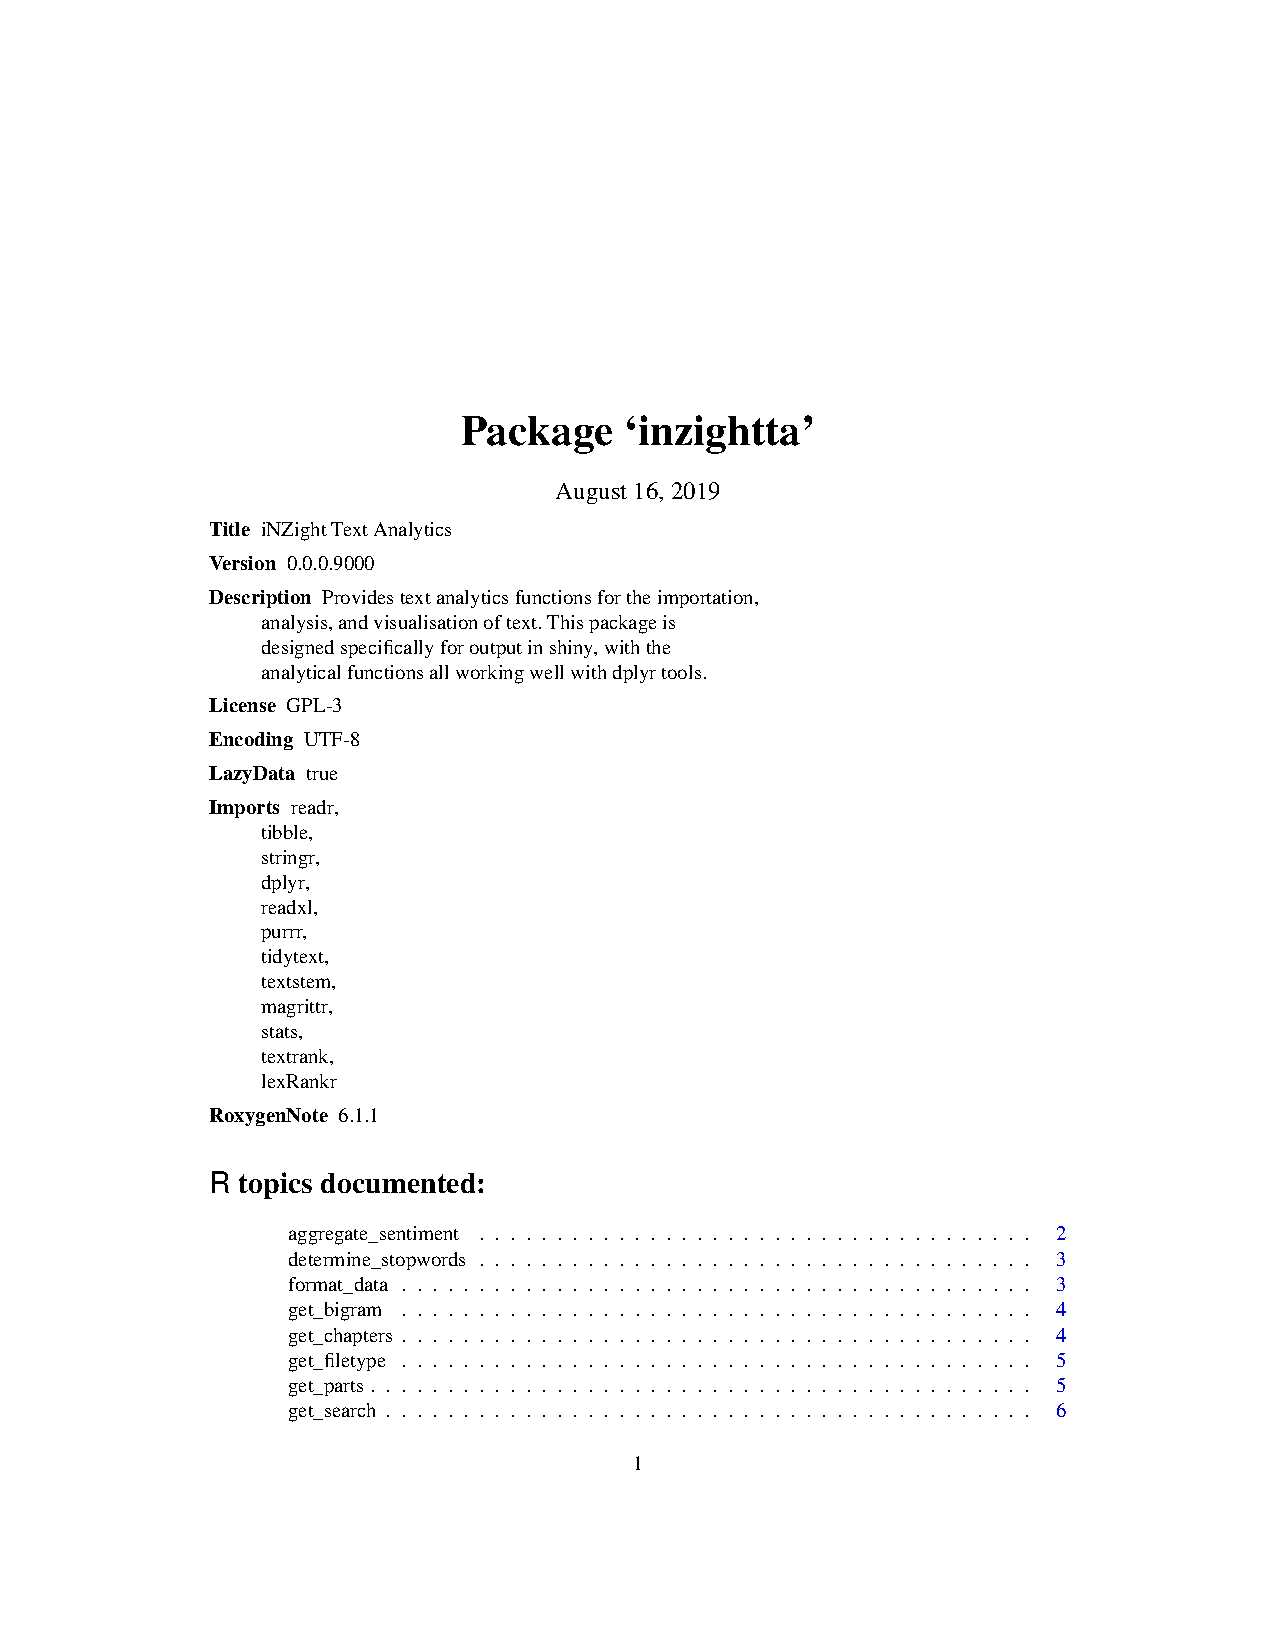
\includepdf[pages=-]{img/inzightta_manual.pdf}

% \backmatter
\addcontentsline{toc}{chapter}{Glossary}
\printglossaries
\addcontentsline{toc}{chapter}{Index}
\printindex
\addcontentsline{toc}{chapter}{Bibliography}
\printbibliography
\end{document}

% \begin{listing}[ht]
% \inputminted[
% frame=lines,
% framesep=2mm,
% fontsize=\footnotesize,
% linenos
% ]{R}{src/table.R}
% \caption{Example Code}
% \label{lst:test}
% \end{listing}

% \begin{table}[ht]
%   \centering
%   \input{src/output_table}
%   \caption{test table}
%   \label{tab:test}
% \end{table}